%TC:envir minted [xx] xxx
\chapter{Verification and validation}

The solution was tested to ensure that it meets all the requirements and provides a bug-free experience.

\section{Testing procedure}

The testing was performed entirely manually. Features were tested as they were developed. The manual incremental approach was chosen due to time considerations. The project is rather small and the result of many operations is a UI rendered from an HTML template, which would make automated testing much more time-consuming. Additionally, the interface had to be visually inspected, so feature testing could be performed as a part of this procedure. Some features such as creating and restarting challenges were tested by either running small scripts or using them via the Node.js REPL and observing results in external tools.

\section{Requirements verification}

The verification of chapter \ref{chap:req-and-tools} requirements fulfilment.

\subsection{Verification of functional requirements}

\begin{enumerate}
	\item \textbf{Account creation}: There is an option to register a new account. Minimum password length is verified both on the client side and on server. It is impossible to register an account with the same username. Additionally, the password has to be typed twice to prevent typos. Stored password is hashed and salted. Accounts are created with the \texttt{"user"} role. The functionality is available under \texttt{/auth/register}. \textbf{Requirement met completely.}

	\item \textbf{Signing in}: Possible through a login page, which is linked in the navbar and on the home page. The functionality is available under \texttt{/auth/login}. \textbf{Requirement met completely.}

	\item \textbf{Logging out}: Users can log out by clicking the logout button, which redirects to \texttt{/auth/logout}. \textbf{Requirement met completely.}

	\item \textbf{Changing password}: Password can be changed on the profile page \texttt{/profile}. The previous password as well as the new password typed twice are required. \textbf{Requirement met completely.}

	\item \textbf{Listing categories}: The list of categories is available in the \textit{Categories} dropdown and on the \texttt{/categories} page. \textbf{Requirement met completely.}

	\item \textbf{Displaying category}: Category pages are provided under \texttt{/category/<name>}. \textbf{Requirement met completely.}

	\item \textbf{Displaying task}: All task properties specified in the requirements are displayed on task pages \texttt{/task/<id>}. \textbf{Requirement met completely.}

	\item \textbf{Solving challenge}: Logged-in users can solve tasks as described in the requirements. \textbf{Requirement met completely.}

	\item \textbf{Answering quiz}: Users who have solved the task challenge can answer the quiz. After answering the correctly marked answers are displayed in green. A summary of correct answers is displayed below the quiz. \textbf{Requirement met completely.}

	\item \textbf{Administrator panel}: Administrator panel is available only for administrators as \texttt{/admin} page. \textbf{Requirement met completely.}

	\item \textbf{Listing users}: The list of users is available under the \textit{Users} tab in the admin panel. The list can also be accessed as JSON as a response to \texttt{GET} request to \texttt{/admin/users} with \texttt{page} and \texttt{size} query parameters. \textbf{Requirement met completely.}

	\item \textbf{Changing user permissions}: User role can be toggled by clicking a button next to the user on the users list. \textbf{Requirement met completely.}

	\item \textbf{Deleting user}: An account can be removed by clicking the red bin icon next to the user on the users list. \textbf{Requirement met completely.}

	\item \textbf{Creating category}: Categories can be created using a form in the \textit{Categories} tab in the admin panel. A \textit{Preview} button can be clicked to toggle between the description input and the preview of rendered HTML. \textbf{Requirement met completely.}

	\item \textbf{Editing category}: Categories can be edited by clicking the \textit{Edit category} button below the category description in the admin panel. The same editor is used for modifying categories as for creating them. \textbf{Requirement met completely.}

	\item \textbf{Creating task}: Tasks can be added as described in the requirements in the \textit{Tasks} tab of the admin panel. \textbf{Requirement met completely.}

	\item \textbf{Starting challenges}: When a task is added, the system automatically starts related challenges. Challenges containers and related nginx configuration are also configured while starting the server. \textbf{Requirement met completely.}
\end{enumerate}

\subsection{Verification of non-functional requirements}

\begin{enumerate}
	\item \textbf{Responsiveness}: The interface has been tested on multiple screen sizes and devices as well as in-browser zoom. The tested native resolutions include: $1920 \times 1080$ (24 in - desktop), $1440 \times 900$ (19 in), $1336 \times 768$ (15.6 in - laptop) and $2400 \times 1080$ (6.67 in - smartphone). Additional screen sizes were tested using the \textit{responsive mode} option in Firefox developer tools. No issues were found during the visual inspection although some answers may cause the viewport to scroll on small screens if they contain specific HTML. \textbf{Requirement met completely.}

	\item \textbf{Accessibility}: There are no accessibility errors in the webhint scan results run from Firefox developer tools. Warning are related to contrast especially in code blocks in light mode. The accessibility results of the scan are presented on Fig. \ref{fig:verify-webhint}. \textbf{Requirement met completely.}

	\item \textbf{Visual consistency}: Styles from the Bootstrap library were used. Additional style sheets follow the Bootstrap colours. Code highlighting follows the theme variant changes (light/dark) and in both modes an appropriate variation of the Panda Syntax theme is used. \textbf{Requirement met completely.}

	\item \textbf{Page load performance}: 98 points performance score in PageSpeed Insights mobile test. Test results are presented on Fig. \ref{fig:verify-perf}. \textbf{Requirement met completely.}

	\item \textbf{Compatibility}: The user interface has been verified to display and work correctly on Firefox, Chrome and Tor Browser (based on Firefox ESR) on Windows, Firefox on Ubuntu and Firefox on Android. Client-side form verification errors are not displayed on Firefox for Android due to \href{https://bugzilla.mozilla.org/show_bug.cgi?id=1510450}{bug 1510450}. Bootstrap dropdowns do not work without JavaScript, so it is impossible to log out or access the profile page with JS disabled. Changing page theme also requires JavaScript, but it is not a core functionality. \textbf{Requirement met partially.}
\end{enumerate}

\begin{figure}
	\centering
	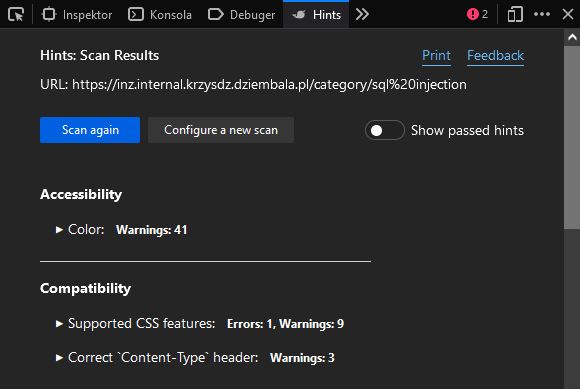
\includegraphics{img/verify-webhint.png}
	\caption{Webhint scan warnings and errors}
	\label{fig:verify-webhint}
\end{figure}

\begin{figure}
	\centering
	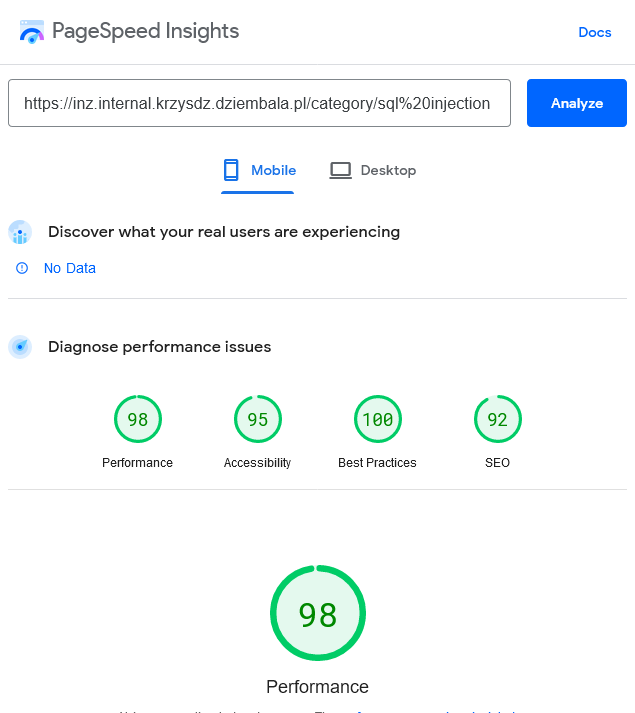
\includegraphics[width=\textwidth]{img/verify-performance-mobile.png}
	\caption{PageSpeed Insights mobile test results}
	\label{fig:verify-perf}
\end{figure}

\section{Detected and fixed bugs}

Most issues were found while writing new features and immediately fixed as a part of adding these features. Some issues, however, slipped through unnoticed and were found and patched separately.

\subsection{Containers were not started at launch if stopped}

If for some reason (e.g. OS restart) challenge containers were stopped while starting the server, these would not be removed and their recreation and start would fail.

The problem was fixed in \href{https://github.com/krzysdz/inz/commit/9fd9017ce994f577233ce0544bbd0cf1df3e0e55}{\texttt{9fd9017}} by ignoring \textit{"container already stopped"} errors when stopping a container.

\subsection{Cookies not set in production}

Cookies were not sent in responses if \mintinline{bash}|NODE_ENV="production"| environmental variable was set. The problem happened, because Express does not send cookies marked as \texttt{secure} if the request was not made with HTTPS. While nginx terminates the external connections with HTTPS, it uses plain unencrypted HTTP to communicate with the server which recognizes it as an insecure protocol.

This problem was fixed in \href{https://github.com/krzysdz/inz/commit/94ca9c4124954c94c9fe8e27dc59305aa59b31ad}{\texttt{94ca9c4}} by setting appropriate headers in the proxy
\begin{minted}{nginx}
proxy_set_header X-Forwarded-Proto $scheme;
proxy_set_header X-Forwarded-For $remote_addr;
\end{minted}
and telling Express to trust the proxy
\begin{minted}[breaklines]{js}
// In production the only way is through nginx, which sets X-Forwarded-For to $remote_addr
if (process.env.NODE_ENV === "production") app.set("trust proxy", true);
\end{minted}
With this change Express recognizes HTTPS connections to the proxy as secure and sends cookies in responses.

\subsection{Unsolved question on task page was escaped}

Task questions should support HTML content and be inserted into template without escaping. In commit \href{https://github.com/krzysdz/inz/commit/b5ae1b16e9be6060b43f28dbb56b090bfb46dd98}{\texttt{b5ae1b1}} support for HTML in questions and answers was added, but this particular place has been overlooked.

The problem was fixed in \href{https://github.com/krzysdz/inz/commit/91128c835889ac0429b478d03c6992541fcdd5c3}{\texttt{91128c8}} with a single line patch:
\begin{minted}[]{diff}
- <h4><%= locals.task.question %></h4>
+ <h4><%- locals.task.question %></h4>
\end{minted}

\subsection{Flag not set as an environmental variable on start}
\label{chap:bug-env-not-set-start}

If \texttt{flagInEnv} was \texttt{true}, the flag would be exposed as an environmental variable when restarting the container, but not after creating it for the first time or restarting the server.

In this instance the problem was fixed in \href{https://github.com/krzysdz/inz/commit/99a0035c61de55ddd7203e7ced1e9fc554959f24}{\texttt{99a0035}} by adding the missing \texttt{Env} option to the \texttt{createContainer} call in \texttt{startChallengeContainer}.

\subsection{Flag not set as an environmental variable for the main challenge}

The \texttt{flagInEnv} option was not saved for the main challenge. The problem was discovered when testing the fix for \ref{chap:bug-env-not-set-start}.

The problem was fixed in \href{https://github.com/krzysdz/inz/commit/f934efb0c50f0156d73bd78fcfcd6a12b5943b1e}{\texttt{f934efb}} by passing the missing option.

\subsection{Task creation fails without additional challenges}

If there were no additional challenges for the incorrect answers, task creation would fail, because \texttt{insertMany()} throws an error if an empty array is passed. There was an empty array check, but it had been implemented incorrectly.

The problem was fixed in \href{https://github.com/krzysdz/inz/commit/f934efb0c50f0156d73bd78fcfcd6a12b5943b1e}{\texttt{f934efb}} by verifying the truthiness of array length instead of the array itself:
\begin{minted}[tabsize=4, obeytabs]{diff}
-		const subChallengeResult = answerChallengeDocs
+		const subChallengeResult = answerChallengeDocs.length
			? await challengesCollection.insertMany(answerChallengeDocs, {
				session,
			})
\end{minted}

\subsection{HSTS header set three times per response}

The \texttt{Strict-Transport-Security} header was sent 3 times with each response. The problem was detected by one of external tools while checking compatibility, accessibility and HTTPS configuration.

The problem was fixed in \href{https://github.com/krzysdz/inz/commit/eec703c98ecb6720c3c2eb0ceee36ca3d7da8aa2}{\texttt{eec703c}} by setting the \texttt{hsts} option of the \href{https://helmetjs.github.io/}{Helmet} middleware to \texttt{false} and removing an \texttt{add\_header} directive from the main configuration, since the shared \texttt{ssl\_common.conf} configuration already contains one.

\subsection{Accounts with \texttt{U+0000} character in username cannot be manipulated by administrators}

Username is used as a part of URI path of account management endpoints. This part of the path is always encoded using \mintinline{js}|encodeURIComponent()| and can be safely sent to the server. Unfortunately, nginx since version 0.8.38 responds with status code 400 if the URI contains a NULL character, even if it is properly encoded. According to Neal Poole the nginx author decided that \enquote{zero byte in URI should not appear in any encoding, operating system, etc., and just makes more problems than helps} and removed support for it in \href{https://hg.nginx.org/nginx/rev/84905c7b2aa7}{changeset 3527} \cite{bib:nginx-null}.

The problem was worked around in \href{https://github.com/krzysdz/inz/commit/0cc6258451fb69f4763be15cf77772b226d2a974}{\texttt{0cc6258}} by forbidding the creation of accounts with the null character in username.
